\documentclass[11pt,twocolumn]{article}
\usepackage[utf8]{inputenc}

\usepackage{a4}
\usepackage{amsmath}
\usepackage{graphicx}
\usepackage{mathtools}
\usepackage{epstopdf}
\usepackage{cuted}
\usepackage{float}
\usepackage{hyperref}
\usepackage{abstract}
\usepackage{subcaption}
\usepackage[toc,page]{appendix}
\usepackage[font=it]{caption}
\usepackage[margin=1.0in]{geometry}
\usepackage{verbatim}

\setlength{\columnsep}{1cm}

\newcommand{\unit}[1]{\ensuremath{\, \mathrm{#1}}}

% MP This gives more space for figures on a page:
\renewcommand{\floatpagefraction}{.95}%


\title{\bf Simulating Tidal Interactions\\ between Galaxies:\\ A Pre-University Student Project}
% MP: Intern could mean a lot of things. Pre-University Student gives people the right idea right away.
\author{
    M. Brea-Carreras, M. Thiel \& M. P\"ossel\footnote{Corresponding author: poessel@hda-hd.de}}
 % MP Date will be added automatically along the side by arXiv
\date{\small Haus der Astronomie, MPIA-Campus, K\"onigstuhl 17, 69117 Heidelberg, Germany	}
% MP: The "Who contributed what" properly belongs in the last section, not here.
% MP: I've put myself as corresponding not least because my e-mail is least likely to change. Will forward any feedback we might receive to you two, of course.
\begin{document}

\maketitle
 \begin{strip}
\begin{abstract}
% MP: Re-wrote this to reflect what I think somebody interested in astronomy education would need to know at this point:
We report on a project undertaken in Summer 2017 by pre-university student interns at Haus der Astronomie: point-particle simulations of galaxy collisions with the aim of reproducing observational data from such collisions. We succeeded in providing a visually similar representation of both NGC 5426/7 and the "Antennae" galaxies (NGC 4038/9), and were able to make deductions about the relative positions and orbits of these galaxies. The project is an example for how participants with little more than high-school level previous knowledge can successfully tackle, and understand, advanced topics from current astrophysical research. This report was written by the two participants (M. B.-C. and M. T.), on whose experiences it is based, in collaboration with their supervisor at Haus der Astronomie (M. P.).
    \end{abstract}
\end{strip}
  
  
\section{Introduction} \label{introduction}
    %%% We probably should start the introduction talking about the educational context, given that it is main focus of the project.
    % MP: I agree that we should begin by talking about context. Have revised accordingly.
There is a broad consensus among science educators about the importance for science education of hands-on activities, elements of inquiry-based learning, and understanding science as a process \cite{Beyond2000,Rocard2007,NRC2011}. For high-school students, or students in limbo between high school and university, internships at research institutions, are a suitable way of experiencing first hand the process of science, whether as part of a larger project or in the course of working on a dedicated student research project.

Haus der Astronomie has offered research internships since 2009, and is currently offering a yearly ``International Astronomy Summer Internship Program'' for advanced high school students, or to students transitioning from high school to college/university.\footnote{Up-to-date information can be found on 
\href{http://www.haus-der-astronomie.de/en/what-we-do/internships/summer-internship}{http://www.haus-der-astronomie.de/en/what-we-do/internships/summer-internship} } Among the authors of this e-print, two of us attended the 2017 internship program (M. B.-C. and M. T.), while one of us was the internship supervisor (M. P.).\footnote{During the first three weeks of the 2017 internship, the project was worked on by M. T. and another intern; during the second three weeks, M. T. and M. B.-C. continued the project in their spare time, on their own initiative. This unusual, and remarkably successful, extra effort prompted M. P. to have the two interns present their results at the WE Heraeus Summer School ``Astronomy From Four Perspectives: The Dark Universe'' in Heidelberg. In summer 2018, this project was also presented by M. T. at the German national teacher training in astronomy at the University of Jena.} 

The project described here used computer simulations to reproduce classic results about galaxy evolution and the observational properties of interacting galaxies. Pedagogically, numerical treatments have several advantages \cite{FeynmanLectures,1978AmJPh..46..748C,1984AmJPh..52..499S}: They allow students to explore dynamical situations that are too advanced for the analytical tools at their disposal; in fact, mathematically, the approach is simpler than many analytical methods. Numerical approaches also allow for a descriptions that are beyond reach for even the most advanced analytical methods. The associated challenge is, of course, that in order to write such simulations themselves (as opposed to using existing software), students need appropriate programming skills.

This e-print serves a double function: For one, it describes the student research project undertaken by M. B.-C. and M. T., to whom the collective ``we'' in the following sections \ref{SummarySection} to \ref{EndProject} refers; this aspect, we hope, will make the text of interest to those involved in astronomy education,
who might be interested in including this or similar student activities in their own programs. In addition, the e-print is part of the project itself. After all, writing up your methods and results is an integral part of scientific work --- even if, in this case, we have included additional aspects related to astronomy education which are not found in ordinary astronomy papers. Each intern presents a personal view of their experiences in the appendix, sections \ref{Brea} and \ref{Thiel}. 

The scripts, simulations parameters and presentations written for this project are publicly available and can be downloaded from GitHub\footnote{The repository can be cloned from
\href{https://github.com/mbrea-c/simulating-tidal-interactions.git}{https://github.com/mbrea-c/simulating-tidal-interactions.git} }.
%The scripts written for this project can be downloaded from d HDA OR DO YOU WANT TO MAKE YOUR OWN GITHUB REPOSITORY?
%MB: We are setting up a Github repository, it should be linked here before next week.
%MB: The repository is up

\section{Project summary}
\label{SummarySection}

Theories of galaxy evolution and formation need to be able to explain, among other things, the appearance of interacting galaxies. The most widely accepted explanation was first studied more intensively in the 1960s \cite{pfleiderer1960spiral}, and identifies tidal interactions between galaxies as the cause of the deformations of the galaxies involved. The main reference for our student research project is a classic 1972 paper by Alar and Juri Toomre  \cite{toomre1972galactic}, which describes basic numerical simulations of galaxy interactions. The authors argue that the bridges and tails visible in some spiral galaxies are remnants of tidal interactions between galaxies involved in a close encounter --- and they support their argument with restricted three-body calculations of selected encounters, including reconstructions of a few well-known pairs: the ``Antennae'' galaxies NGC4039/39, the ``Mice'' galaxies NGC 4676, and M51 with its small companion NGC 5195. 

For our research project, we followed in the footsteps of Toomre and Toomre by creating our own galaxy simulation, written using the Python programming language.\footnote{Python Software Foundation. Python Language Reference, version 2.7. Available at \href{http://www.python.org}{http://www.python.org}} We describe our simulation techniques in section \ref{methods}, while section \ref{simulations} presents our results. In section \ref{education}, we draw on our personal experience to give recommendations for similar educational projects. 

% MP: Could you make more clear at this point what part of the work was in 2D, and what in 3D?
% MB: Sure, we will specify more in the methods section. It was a 3D simulation in every case in the sense that a third dimension was supported by our code and taken into account for the calculations; however, in the first two examples, both galaxies share the same orbit plane and their movement is always parallel to said orbit plane (they are in effect equivalent to a 2D simulation, the z-coordinate is alway zero for every particle)
% MP: OK!
 \section{Methods} \label{methods}

Our simulations were written in Python. We are aware that using a general programming language like Python as the basis of a student research project will raise the bar higher than reliance on more specialized and restricted software for students unfamiliar with programming; in our case, one of us (M. B.-C.) had previous experience in using Python, while the other (M. T.) learned Python during his internship, but had some previous experience programming in Java. Going by our personal experience, we think that Python is a good choice for those who are new to programming.

The simulations were all three-dimensional, in the sense that all vector data stored and used in the computations was three-dimensional. However, in the first two examples all particles and velocities are confined to the same plane, making those simulations two-dimensional in effect.



The basic elements of our physical model are point particles with mass on the one hand and point particles without mass on the other hand. The latter serve as test particles, which are acted upon by gravitational forces but are not themselves treated as sources of gravity. Following Toomre and Toomre, the mass of each galaxy is represented by a single point particle with the total galaxy mass, which is located in the center of the galaxy. Galaxy structure is simulated using test particles representing stars in each galaxy's (initially undisturbed) disk. 
        
        
Thus, in a two-galaxy simulation we have just two sources of gravity: the two central point particles carrying each galaxy's mass. For all other particles, we only need to calculate how they react to the gravitational forces exerted by the two central point particles. 
 
        % MP: Your initial version sounded as if you gave the test particles a mass, as well - but you didn't, right? 
        % MB: Right, it was a mistake (it was made clear in another part of the text that we later moved). Changed accordingly.
        % MP: OK!
        
       These core elements require only their three-dimensional position and velocity information to be stored --- and, in the case of the central particle of each galaxy, their scalar mass. This data, along with a predefined time-step, is passed to an update function, which returns the particles' new positions and velocities. Results are plotted using the Python 2D plotting library matplotlib \cite{Hunter:2007}, which we found simple and straightforward to use for our purposes.
% MP: the "2D plotting library" is the official matplotlib description. I assume even with 3D plots, what matplotlib gives you is a 2D projection.
%
% MP: I moved the variable details below. Always better to talk about the physics first, the implementation later.
        
        \subsection{Update Function}
        
        In order to define a physical update function for a simulation -- which encapsulates how our system changes over time -- we need to perform a second order integration: to solve for the trajectory of moving bodies affected by a location-dependent acceleration. Whereas the two-body problem for two point particles orbiting each other under the influence of their mutual gravitational attraction can be solved analytically, the general situation of three or more bodies can only be described numerically.
        
 % MP I've fleshed this out a bit. Always define your terms, and describe where everything comes from.
 
 % MB: Should we change the notation to using boldface for vectors instead of an arrow? I think it would make the equations clearer, but I haven't found any consistent information on vector variable typesetting so I'm not sure what's the standard way to do it in astronomy.
 % MP: I don't think there is a standard way of doing this. Vectors with arrows should be fine.
In our particular set-up, we have $N$ particles, each designated by an index $j$. We denote the $j$th particle's position at time $t$ as $\vec{x}_j(t)$, its velocity at time $t$ by $\dot{\vec{x}}_j(t)$ and its acceleration by $\ddot{\vec{x}}_j(t)$. The acceleration felt by the $j$th particle at time $t$ results from the sum of all the other particles exerting a gravitational force; each separate gravitational influence is described by Newton's inverse-square law of gravity. The total acceleration of the $j$th particle is 
        \begin{equation}
                \ddot{\vec{x}}_j(t) =- G\sum_{i \neq j} m_i\cdot  \frac{\vec{x}_{j}(t) - \vec{x}_{i}(t)\phantom{{}^3}}{|\vec{x}_{j}(t) - \vec{x}_i(t)|^3},
                \label{GravitationalAcceleration}
        \end{equation}
 where $m_i$ is the mass of the $i$th particle and $G$ denotes the gravitational constant. As our test particles are massless, they can be skipped in the summation. Only the "galaxy centers of mass" need to be taken into account when computing the acceleration of any particle $j$.
 
For the purpose of numerical integration, time is divided into discrete time steps. The update function is used to calculate the state of the system after each additional time step, based on the information available at the present time step or earlier time steps. We define the elapsed time at time-step $n$ as
         \begin{equation}
         t_n = t_0 + n h
         \end{equation}
where $h$ denotes the (in our case: universal) time interval between one time step and the next. This discretisation is a simplification, and it stands to 
reason that the value defined for $h$ will have direct consequences for the accuracy of any numerical calculation.
        
        
            \subsubsection{Euler method}
            
            	\begin{figure}
                \centering
  				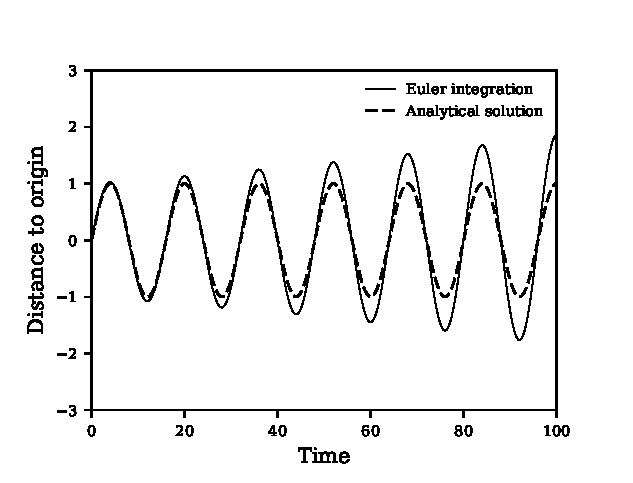
\includegraphics[width=0.5\textwidth]{num_st/euler.eps}
  				\caption{Displacement from origin over time using Euler integration method (step length $h = 0.08$), compared with the
                analytical solution for a simple harmonic oscillator with amplitude $A = 1$ and angular frequency $\omega = \frac{\pi}{8}$.}
  				\label{fig:euler}
				\end{figure}
                
                The most straightforward way of numerical integration is the Euler method, in which all rates of change are approximated as linear, and the change in a function is taken to be the rate of change times the duration of the time step. Following this prescription, the Euler integration algorithm computes the updated velocity and position for each body $j$ and for each iteration $n$  as           
              %  \setcounter{equation}{0}
              % MP: It's good practice to count equations from the beginning to the end. That way, if someone wants to refer to an equation, they only
              % need to know which paper, and a single number.
              % Also, for two equations directly following each other, use eqnarray
                \begin{eqnarray}
                \dot{\vec{x}}_j(t_{n+1})& =& \dot{\vec{x}}_j(t_n) + h \ddot{\vec{x}}_j(t_n)
                \label{EulerAcceleration}\\[0.5em]
                \vec{x}_j(t_{n+1})& =& \vec{x}_j(t_n) + h \dot{\vec{x}}_j(t_n),
                \end{eqnarray}
                where $n$ is the number of iterations, and thus $n h$ is the elapsed time. At each step, we need to determine each particle's acceleration vector $\ddot{\vec{x}}_{j}(t_n)$ following equation (\ref{GravitationalAcceleration}).
                
			\subsubsection{Numerical errors and the velocity Verlet Algorithm}
			\label{StabilitySection}
			Euler integration incorporates certain systematic errors, which lead to cumulative divergence between a numerical solution and the true solution. An instructive example is that of the one-dimensional harmonic oscillator, where the acceleration is given by
			\begin{equation}
			\ddot{x} = -\omega^2 x
            \label{Hooke}
			\end{equation}
			(Hooke's law) for some constant angular frequency $\omega$. In this simple case, we can directly write down an analytical solution 
			\begin{equation}
			x(t)  = A\cdot \sin(\omega t),
			\end{equation}
			with $A$ the amplitude of the oscillation. This allows for a direct comparison between the analytical and numerical solution which exposes some of the problems inherent in numerical simulations.			
			Imagine that the moving mass of that oscillator is moving towards positive $x$, so that  we are in an phase where $\dot{x}>0$. 
			The Euler prescription (\ref{EulerAcceleration}) assumes that the acceleration acting on our mass during the time step $t_n$ is equal to the acceleration at the {\em beginning} of that time step. But in reality, we know that the effect of the acceleration will be greater than that. After all, during that time step, the mass is moving towards greater x, and the acceleration pulling it back will increase at greater x values. Evidently, the Euler method systematically underestimates the pull experienced by our mass. Conversely, when our mass is moving back towards the origin, the Euler method will systematically overestimate the pull. Both effects erroneously increase the total energy, and thus the amplitude, of the oscillation: the first since it allows the mass to move further outward than allowed, and the second because it imparts a larger momentum on the mass. The cumulative effect can be seen in figure \ref{fig:euler}, where the numerical solution progressively diverges from the analytical solution. 
			
Such integration errors have led to the development of alternative numerical integration schemes. One such scheme is the velocity Verlet algorithm \cite{1967PhRv..159...98V}.
                \begin{figure}
                \centering
  				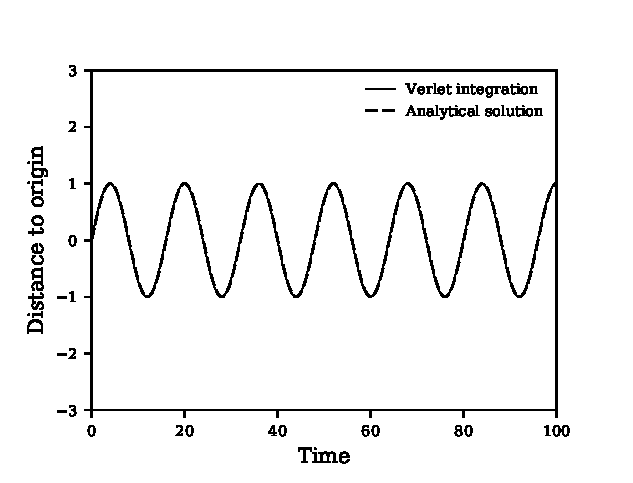
\includegraphics[width=0.5\textwidth]{num_st/verlet.eps}
  				\caption{Displacement to origin over time using Verlet integration method ($h = 0.08$) against the analytical solution of a simple harmonic oscillator $x(t) = A\cdot\sin(\omega t)$, with $A = 1$ and $\omega = \frac{\pi}{8}$).}
  				\label{fig:verlet}
				\end{figure}         
This method introduces additional ''half-steps'' for time, which we will designate by $t_{n+1/2} = (n+1/2)h$. First, the velocity is calculated at one such half-step as
                \begin{equation}
                \dot{\vec{x}}_j(t_{n+1/2}) = \dot{\vec{x}}_j(t_n)  +  \frac{h}{2} \ddot{\vec{x}}_j(t_n)
                \end{equation}
where the acceleration is of course system-specific, eq. (\ref{Hooke}) in the case of the harmonic oscillator, or eq. (\ref{GravitationalAcceleration}) for our galaxy simulation. Once computed, this half-step velocity is used to find the position at $t_{n+1}$ as                 
\begin{equation}
                {\vec{x}}_j(t_{n+1}) = {\vec{x}}_j(t_n) + h\dot{\vec{x}}_j(t_{n+\frac{1}{2}}) 
                \end{equation}
                Next, using these newly-determined position values, the acceleration {\em evaluated at} $t_{n+1}$ is computed, and used to 
                compute  $\dot{\vec{x}}_{n+1}^{(j)}$, as                
                \begin{equation}
				\dot{\vec{x}}_j(t_{n+1}) = \dot{\vec{x}}_j(t_{n + \frac{1}{2}}) + \frac{h}{2} \ddot{\vec{x}}_j(t_{n+1}).
                \end{equation}
For the simple example of the harmonic oscillator, the comparison between figures \ref{fig:euler} and \ref{fig:verlet} shows the remarkable increase in numerical stability of this improved algorithm --- at least within the range of the simulation shown in those figures, the Verlet version does not visibly overshoot the mark! The increase in computational cost is a mere 50\%, as the half-steps are used only in the velocity calculation, not in the position calculation.
           
        \subsection{Initial values }
        % MP: We need to motivate why this is here in the first place. It's a general property of solving differential equations.
The algorithms described in the previous two sections allow us to simulate the {\em evolution} of physical systems. In order to pick out a particular solution, we need to specify appropriate initial values, as is generally the case when solving differential equations.

The aim of our project is to simulate interactions between galaxies; our initial conditions amount to modelling, in an appropriate way, the original two galaxies involved in the interaction. We make the assumption that, before the interaction proper, we can regard the galaxies as completely separate systems. For each of the galaxies, the test particles are assumed to be in circular orbit around the central galaxy particle.

\subsection{The  two-body problem} \label{rmin}

Since we have only the two central particles acting as sources of gravity, it is possible to calculate their motion analytically --- after all, the two-body problem allows for direct analytical solutions. We have made use of this analytical description in choosing the initial conditions for the two central particles, computing the orbital eccentricity $e$ and eventual pericenter distance $R_{min}$ (that is, the distance of closest approach of the galaxy point partices) in each case. 

The key concepts and equations are as follows \cite[chapter 9]{1965mech.book.....K}: Due to the conservation of angular momentum, the two-body motion takes place in the two-dimensional plane defined by the two initial velocity vectors of the central point particles. 
        % Possibly make more clear where we switch to polar coordinates
        % MP: Have tried to add a bit about this later on.
        
For two centers of mass $m_1$ and $m_2$ with positions $\vec{x}_1$ and $\vec{x}_2$, relative position $\vec{r}$ and reduced mass $\mu$ are defined as 
        \begin{equation}
        \vec{r} = \vec{x}_2 - \vec{x}_1
        \end{equation}
        and
        \begin{equation}
        \mu = \frac{m_1 m_2}{m_1 + m_2},
        \end{equation}
        respectively.
Solving the two-body problem amounts to solving two one-body problems: free, linear motion for the center-of-mass of the system, and an effective one-body problem for the relative motion of a particle of mass $\mu$ with position vector $\vec{r}$ in the Newtonian potential of a point mass $M=m_1+m_2$; this latter motion results in a Kepler ellipse. Using polar coordinates $(r,\theta)$, with the origin located at one of the focus points, the shape of the ellipse is described by 
   \begin{equation}
        r = \frac{r_0}{1 - e \cos\theta}.
        \label{EllipseEquation}
        \end{equation}
Here, $\theta=0$ corresponds to the direction from the focus to the center of the ellipse; $e$ is the ellipse's eccentricity.
The quantity $r_0$ is called the {\em semilatus rectum} and sets the length scale of the ellipse.

Each orbit is characterized by two conserved quantities: the mechanical energy
\begin{equation}
        E = \frac{1}{2}\mu \dot{r}^2 - \frac{G m_1 m_2}{r}=\frac{1}{2}\mu \dot{r}^2 - \frac{G \mu M}{r}
        \end{equation}
 and the angular momentum
 \begin{equation}
        L = \mu\cdot \dot{r}_{trans} \cdot r,
        \end{equation}
where $\dot{r}$ is the relative speed of the two centers of mass and $\dot{r}_{trans}$ the component of the relative velocity that is transversal to the location vector.
        
Using $E$ and $L$, the two parameters in equation (\ref{EllipseEquation}) for the shape of the elliptical orbit can be written as
       \begin{eqnarray}
        r_0 &=& \frac{L^2}{\mu G m_1 m_2}\\[0.5em]
        e\phantom{{}_0} &=& \sqrt{1 + \frac{2 E L^2}{\mu (Gm_1m_2)^2}}.
        \end{eqnarray}
Computing the minimal distance $R_{min}$ of our $\mu$ particle from the center of attraction, which is also the minimal distance between our two galaxy particles, amounts to solving an optimization problem, namely
        \begin{equation}
        \frac{\mathrm{d}r}{\mathrm{d}\theta} = \frac{r_0}{1 - e\cos\theta} (e\sin\theta) \stackrel{!}{=}0.
        \end{equation}
The result is      
 \begin{equation}
       \sin\theta = 0.
       \end{equation}
Since $0 \leq \theta < 2\pi$, we must have either $\theta = 0$ or $\theta = \pi$. Inserting these values into (\ref{EllipseEquation}), we find that the minimal value is at $\theta=\pi$, namely
         \begin{equation}
       R_{min} = \frac{r_0}{1 + e}.
       \end{equation}
In our attempts to model certain specific interactive pairs of galaxies, we made use of this relation in choosing (albeit with a certain amount of trial and error) suitable initial values.

\subsection{Optimization}
\label{Optimization}
% MP: I have consolidated several sections under this overall heading.

Even with computers inordinately more powerful than in the early 1970s, when Toomre and Toomre created their simulations, run time values and run time differences in our Python scripts were notable features of our project --- and just like in professional simulation projects, we experimented with ways of optimizing the performance of our programs. 

One area where different implementations turned out to make a considerable difference involved different ways of storing our simulation data. The simplest way of handling simulation data, which we would recommend for students with little to no programming experience, involves the use of Python list objects. The simulation itself involves iterative loops that wrap the update function. 

This implementation turns out to be comparatively slow. In those of our simulations that involved a considerable number of test particles, run time did set the pace both for testing our programs and for finding the best initial values. 

As an alternative, we took advantage of the array structures and associated linear algebra functionality of the NumPy core package within the SciPy ecosystem for Python \cite{SciPyLibrary,NumPy}. User-defined functions such as those necessary to implement our update function can be ''vectorized'' to allow their direct application to array objects, eliminating the need for explicit loops. The linear algebra aspect of that alternative makes it somewhat more challenging for a high school project, but if it is included, the pay-off is a substantial gain in speed, as shown in table \ref{table:extimes}.
            \begin{table}[ht]
            \centering
            \bgroup
            \renewcommand{\arraystretch}{1.2}	
            \begin{tabular}{r | r | r}
            $m$ & Non-vectorized & Vectorized \\ \hline
            28  & 11.291\,s &  1.42\,s \\ 
            134 & 45.404\,s &	 1.511\,s \\
            202 & 67.753\,s &  1.597\,s \\
            268 & 85.136\,s &	 1.621\,s \\
            406 & 126.231\,s & 1.763\,s \\
            540 & 166.262\,s & 1.915\,s \\
            676 & 206.818\,s & 1.993\,s \\
            810 & 251.798\,s & 2.123\,s \\
            \end{tabular}
            \egroup
            \caption{Execution times for increasing particle count $m$ for a constant number of 5000 time steps.
                        \label{table:extimes}}
            \end{table}
In accordance with good computing practices, we also experimented with an object-oriented approach to programming our simulation, as a way of keeping the code modular and easier to organise and debug. In the end though, we found it difficult to reconcile a fully object-oriented approach with the vectorisation of our variables and the update algorithm. 
        
        	%OLD TEXT (((There are two main potential approaches for the implementation of these core items. The most elementary approach, and probably best to try with students who have not programmed before, is to use arrays to store velocity, position, and mass where relevant. This way, the hassle of introducing students to object-oriented programming can be avoided, and opportunities to better vectorize the code further down the line might appear more obvious, even if it is also possible using objects.
            
            %More dedicated students, however, might want to go one step further and dive into the more advanced object-oriented approach. If implemented right, it can help keep your code clean --for those that understand the concept of OOP--, and be helpful when debugging and adding new features. That is, of course, because an object-oriented implementation requires the code to be modular to a certain extent. An object oriented approach also allows for vectorization, but again, it might not seem as obvious to someone new to programming.))) OLD TEXT % 
       
            
            % Is this part too personal? (mentioning our expectations being exceeded). It should probably be changed.
            % (OLD TEXT)Taking advantage of the linear algebra libraries present in the NumPy module in the implementation of the relevant update algorithm is an issue that earned its own subsection, as the results it provided are truly astounding.

            %(OLD TEXT) There was never a doubt that a vectorized implementation would bring a great improvement to performance, but the measured simulation times exceed the expectations, as Figure \ref{fig:extimes} shows.
            
            
            % (OLD TEXT)These improvements were a key factor in the search for adequate parameters for the documented simulations, as they allowed for faster simulation testing. Furthermore, being able to run simulations faster also sped up the debugging process, and it made possible to increase the amount of particles by orders of magnitude (see Figure \ref{fig:ngc5426} at $t=22$, where the total particle count has been set to $76856$) %Maybe round that number
            
            %(OLD TEXT) On another note, the vectorization of the code will open the door for the implementation of N-body simulations, which require far greater computational power. 
            
            %(OLD TEXT) Withal, it should be considered whether it is adequate or not as an extra task for the students working on this project, as it would involve a sizable amount of research on their part and some acceptable final results can be reached without it.
            
Last but not least, creating the diagrams used to display the results of our simulations proved a significant contribution to overall run time. We made use of the Matplotlib library \cite{Hunter:2007} for this purpose, which uses the CPU for displaying graphics and thus has a substantial impact on performance. This impact can be reduced when rendering only each $n$th frame, e.g. only every $10^8$ or $10^7$ years of simulated time. An alternative possibility for optimisation, which we did not attempt but which might be of interest to others, would be to switch to 
VPython or PyOpenGL,\footnote{
Information can be found on \href{http://vpython.org/}{http://vpython.org/} and 
\href{http://pyopengl.sourceforge.net/}{http://pyopengl.sourceforge.net/}, respectively.} both of which are GPU-based.
            

            %(OLD TEXT) Nevertheless, given that matplotlib uses the CPU for displaying graphics, it quickly becomes a performance bottleneck. It is thus very important to consider the amount of frames that are to be rendered, which do not have to match the number of physics time-steps. In our simulations, we have plotted a frame every iteration when the elapsed time reaches a multiple of $10^8$ years if taking individual images, and $10^7$ years when making a movie of the simulation.

\section{Simulations} \label{simulations}
    
The simulations we created for our project were of two types: in our first step, we set out to replicate two of what Toomre \& Toomre call their  ''elementary examples'' \cite[section II]{toomre1972galactic}, namely the retrograde passage and the direct passage of a small companion. In both cases, there is a main galaxy modelled as a central particle surrounded by a flat disk of orbiting test particles, while the second galaxy is modelled only as a single central particle. In these encounters, the orbital plane of the two central particles coincides with the disk plane of the main galaxy, so the situation as a whole is confined to a two-dimensional plane.

The main part of our project was then dedicated to simulating the interactions in the NGC 5426/7 system and for the "Antennae" (NGC 4038/9) pair of galaxies. In these simulations, each of the interacting galaxies has a disk of orbiting stars, modelled as a disk of test particles, but the simulation is no longer restricted to a two-dimensional plane.
% MP: And they are, presumably, three-dimensional  - mention this?
% MB: We changed the text to specify that.
    
    %(OLD TEXT) The amount of particles used varied throughout the examples; it has been increased in some cases to make the results more apparent.
        
        
        \subsection{Retrograde passage of a equal-mass companion}

            \begin{figure}[!htbp]
            \captionsetup[subfigure]{labelformat=empty}
  			\begin{subfigure}[b]{0.2\textwidth}
    			\includegraphics[width=\textwidth]{fig_1/Fig3_1_000000_0.pdf}
    			\caption{$t = 1$}
  			\end{subfigure}
  			\hfill
  			\begin{subfigure}[b]{0.2\textwidth}
    			\includegraphics[width=\textwidth]{fig_1/Fig3_2_000000_0.pdf}
    				\caption{$t = 2$}
  			\end{subfigure}
            \hfill
            \begin{subfigure}[b]{0.2\textwidth}
    			\includegraphics[width=\textwidth]{fig_1/Fig3_3_000000_0.pdf}
    				\caption{$t = 3$}
  			\end{subfigure}
            \hfill
            \begin{subfigure}[b]{0.2\textwidth}
    			\includegraphics[width=\textwidth]{fig_1/Fig3_4_000000_0.pdf}
    				\caption{$t = 4$}
  			\end{subfigure}
  			
            \begin{subfigure}[b]{0.2\textwidth}
    			\includegraphics[width=\textwidth]{fig_1/Fig3_5_000000_0.pdf}
    				\caption{$t = 5$}
  			\end{subfigure}
            \hfill
            \begin{subfigure}[b]{0.2\textwidth}
    			\includegraphics[width=\textwidth]{fig_1/Fig3_6_000000_0.pdf}
    				\caption{$t = 6$}
  			\end{subfigure}
            \hfill
            \begin{subfigure}[b]{0.2\textwidth}
    			\includegraphics[width=\textwidth]{fig_1/Fig3_7_000000_0.pdf}
    				\caption{$t = 7$}
  			\end{subfigure}
            \hfill
            \begin{subfigure}[b]{0.2\textwidth}
    			\includegraphics[width=\textwidth]{fig_1/Fig3_8_000000_0.pdf}
    				\caption{$t = 8$}
  			\end{subfigure}
            \caption{Flat retrograde passage of a companion with equal mass, simulated with $120$ particles. Both the main galaxy and the companion have a mass of $10^{11}\: M_\odot$. All time values are given in multiples of $10^8\:$ years. In this example, $e \approx 1.21$ and $R_{min} \approx 30.46 \unit{kpc}$.}
            
            %\caption{Flat retrograde passage of a companion with equal mass. Both the main galaxy and the companion have a mass of main galaxy mass $10^{11}\: M_\odot$ and contain 120 particles. All time values are given in multiples of $10^8\:$ years. In this example, $e \approx 1.21$ and $R_{min} \approx 30.46 \unit{kpc}$.}
            \label{fig:fig3}
		\end{figure}
Figure \ref{fig:fig3} shows two galaxies with equal masses. One of the galaxies has a ring of test particles; we observe how those test particles react to the passage of the second galaxy. The orbit of the perturbing body is retrograde with respect to the revolution of the first galaxy's particles, in other words: the sense of rotation of the second galaxy's orbit is opposite to the sense of rotation of the test particles in the rings of the first galaxy.

%(OLD TEXT)This passage is considerably hyperbolic with $e \approx 1.21$ and $R_{min} \approx 30.46 \unit{kpc}$ compared to Toomre \& Toomre's exact parabolic encounter \cite{toomre1972galactic} with an eccentricity of $e = 1$ and eventual pericenter distance of $R_{min} =  25 \unit{kpc}$
    
    % We might want to remove this paragraph, as it feels like mostly stating the obvious..
    % MP: I would leave the (following) paragraph in!
As seen at $t = 3\cdot 10^8\:$years and onwards, only the outermost rings show obvious perturbations in their orbit. This results in the formation of a galactic tail at $t = 5\cdot 10^8\:$years, which dissipates soon after. The result is similar to that of Toomre \& Toomre  \cite{toomre1972galactic}. A small difference, namely the extent of the outermost regions of the disk at $t=5\cdot 10^9\:$years, is readily explained by differences in the initial values.
        
\subsection{Direct passage of a smaller companion}
        
        In this example, we are again looking at a galaxy with test-particle ring. This time, the passing companion has a mass only a quarter that of the first galaxy. Furthermore, this is a \textit{direct} passage: the sense of rotation of the passing companion's orbit relative to the first galaxy is the same as the sense of rotation of the test particles in the first galaxy's rings. The resulting encounter is shown in figure \ref{fig:fig4}. A prominent feature of this encounter is the formation of a bridge between the main galaxy and the companion. The bridge does not last very long, however. By the time the simulation has reached about $t=12\cdot 10^8\:$years, this bridge has dissipated completely. Notably, this means the bridge is much shorter-lived than the tidal counter-arm that has also been produced in the encounter.          %(OLD TEXT) These values are, however, considerably closer to Toomre \& Toomre's values than those in the previous example, which makes us expect a result also closer to theirs. A larger amount of particles is used here, aiming to help with the observation of the resulting bridge.
        
           \begin{figure*}[!htbp]
        \captionsetup[subfigure]{labelformat=empty}
  			\begin{subfigure}[b]{0.2\textwidth}
    			\includegraphics[width=\textwidth]{fig_4/Fig4_4_000000_0.pdf}
    			\caption{$t = 4$}
  			\end{subfigure}
  			\hfill
  			\begin{subfigure}[b]{0.2\textwidth}
    			\includegraphics[width=\textwidth]{fig_4/Fig4_6_000000_0.pdf}
    				\caption{$t = 6$}
  			\end{subfigure}
            \hfill
            \begin{subfigure}[b]{0.2\textwidth}
    			\includegraphics[width=\textwidth]{fig_4/Fig4_7_000000_0.pdf}
    				\caption{$t = 7$}
  			\end{subfigure}
            \hfill
            \begin{subfigure}[b]{0.2\textwidth}
    			\includegraphics[width=\textwidth]{fig_4/Fig4_8_000000_0.pdf}
    				\caption{$t = 8$}
  			\end{subfigure}
  			
            \begin{subfigure}[b]{0.2\textwidth}
    			\includegraphics[width=\textwidth]{fig_4/Fig4_9_000000_0.pdf}
    				\caption{$t = 9$}
  			\end{subfigure}
            \hfill
            \begin{subfigure}[b]{0.2\textwidth}
    			\includegraphics[width=\textwidth]{fig_4/Fig4_10_000000_0.pdf}
    				\caption{$t = 10$}
  			\end{subfigure}
            \hfill
            \begin{subfigure}[b]{0.2\textwidth}
    			\includegraphics[width=\textwidth]{fig_4/Fig4_11_000000_0.pdf}
    				\caption{$t = 11$}
  			\end{subfigure}
            \hfill
            \begin{subfigure}[b]{0.2\textwidth}
    			\includegraphics[width=\textwidth]{fig_4/Fig4_12_000000_0.pdf}
    			\caption{$t = 12$}
                \label{fig:fig4h}
  			\end{subfigure}
            
            %\caption{Flat direct passage of a smaller companion, simulated with $120$ particles per galaxy: main galaxy mass $10^{11}\: M_\odot$, companion galaxy mass $2.5 \cdot 10^{10}\: M_\odot$. All time values are in multiples of $10^8\:$ years.
            
            \caption{Flat direct passage of a smaller companion, simulated with $120$ particles: main galaxy mass $10^{11}\: M_\odot$, companion galaxy mass $2.5 \cdot 10^{10}\: M_\odot$. All time values are in multiples of $10^8\:$ years.
            The orbital parameters are $e \approx 1.04$ and $R_{min} \approx 27.02\unit{kpc}$.} %Again, we might want to compare it to Toomre's
            \label{fig:fig4}
		\end{figure*}
		
% MP: I find it hard to keep track of the companion in these diagrams. Presumably it is at the arrow tip at t=3? Or is it at the base of the arrow? And out of view in all subsequent frames?
% MB: We increased the particle size and line width to make it more clear when the companion is shown in the frame.
        
    \subsection{Three-dimensional model of NGC 5426}

The galaxy pair consisting of NGC 5426 and NGC 5427, which is shown in figure \ref{NGC5426n7}, is a remarkable example of spiral arms and a bridge forming due to tidal interactions. As part of our project, we attempted to recreate these structures. 
\begin{figure}[htbp]
\begin{center}
\includegraphics[width=\linewidth]{ngc5426/gemini-ngc5426n7small.jpg}
\caption{The galaxy pair NGC 5426 and 5427. Image credit: Gemini Observatory/Association of Universities for Research in Astronomy}
\label{NGC5426n7}
\end{center}
\end{figure}
        
        % (OLD TEXT) Even though the two galaxies appear to be just next to each other at plain sight, the possibility that NGC 5426 is well behind its companion has to be considered. Along these lines, we set up the simulation so that the passage resulted sub-parabolic ($e \approx 0.67$), but maintaining a reasonably high eventual pericenter distance ($R_{min} \approx 28.16 \unit{kpc}$). Regarding the inclination, it can clearly be observed that the angle of inclination is considerably smaller for NGC 5427.
        
In the encounter we simulated, the revolution of the particles were retrograde to the orbit of the interacting galaxies with each other. The results of our simulation can be seen in figure \ref{fig:ngc5426}. From the chosen perspective, NGC 5426 has initially started on the left side of the view. By the time $t=7\cdot 10^8\:$years, the first close encounter has already occurred, and NGC 5426 can be seen to the right of its companion.

In the snapshot at  $t=7\cdot 10^8\:$years, one can see the bridge connecting the two galaxies. 
        
In the snapshots at $t=7\cdot 10^8\:$years and $t=12\cdot 10^8\:$years, both galaxies are moving away from each other, and are approaching their apocenters by $t=22\cdot 10^8\:$ years.

% MP: What is meant by the following sentence? What is the surprising part, what is expected, what is neither?
% MB: We will take a look at the whole results section again, the text is not very clear right now.
% (OLD TEXT) Thus, in our model, we find that NGC 5426 is not only not as close as expected to its companion, but they are almost the furthest they will ever be in their current orbit.
        
At $t=22\cdot 10^8\:$years the simulated galaxies share visual similarities with their observed counterparts: global spiral arms similar to those in the observed galaxies are present.
        
        \begin{figure*}[!tbp]
        \captionsetup[subfigure]{labelformat=empty}
        	
            \begin{subfigure}[b]{0.45\textwidth}
    			\includegraphics[width=\textwidth, trim={1cm 6cm 1cm 6cm}, clip]{ngc5426/Ngc2_000000_115.pdf}
    			\caption{$t = 2$}
  			\end{subfigure}
            \hfill%%
            \begin{subfigure}[b]{0.45\textwidth}
    			\includegraphics[width=\textwidth, trim={1cm 6cm 1cm 6cm}, clip]{ngc5426/Ngc7_000000_115.pdf}
    			\caption{$t = 7$}
  			\end{subfigure}
            \centering
            \begin{subfigure}[b]{0.9\textwidth}
    			\includegraphics[width=\textwidth, trim={0cm 5.5cm 0cm 5.5cm}, clip]{ngc5426/Ngc12_000000_115.pdf}
    			\caption{$t = 12$}
  			\end{subfigure}
%%%%%%%%%%%%%%%%%%%%%%%%%%%%%%%%%%%%%%%%%%%%
			
            \begin{subfigure}[b]{0.9\textwidth}
\includegraphics[width=\textwidth, trim={0cm 5.5cm 0cm 4cm}, clip]{ngc5426/Ngc22_000000_115.pdf}
    			\caption{$t = 22$}
  			\end{subfigure}%%%%%%%%%%%%%%%%%%%%%%%%%%%%%%%%%%%%%%%%%%%%
            
            \caption{Simulated interaction between galaxies analogous to NGC 5426 and NGC 5427, with a total of $75000$ particles ($37500$ on each galaxy's initial disk). The encounter was a retrograde passage where both galaxies had equal mass. The projection plane formed and angle of $83^{\circ}$ with the two central particles' orbital plane. The two particle disks have a relative inclination of $30^{\circ}$ with respect to each other. In this simulation, the eccentricity of the orbit is $e \approx 0.67$ and the distance of closest approach is $R_{min} \approx 28.16 \unit{kpc}$.}
            \label{fig:ngc5426}
            
            %\caption{Simulated interaction between galaxies analogous to NGC 5426 and NGC 5427, with a toal of $75000$ particles ($37500$ on each galaxy's initial disk). The encounter was a retrograde passage where both galaxies had equal mass. The projection plane formed and angle of $83^{\circ}$ with the two central particles' orbital plane. The two particle disks have a relative inclination of $30^{\circ}$ with respect to each other. In this simulation, the eccentricity of the orbit is $e \approx 0.67$ and the distance of closest approach is $R_{min} \approx 28.16 \unit{kpc}$.}
            \label{fig:ngc5426}
		\end{figure*}

        
        %\subsection{A Three-Dimensional Model of the Mice Galaxies (NGC 4676)}
        % Add this or no?
        
        \subsection{Antennae galaxies NGC 4038/9}
    \begin{figure}[htbp]
\begin{center}
\includegraphics[width=\linewidth]{Antennae/noao-kittpeak-antennae.jpg}
\caption{Visible-light observation of the antennae galaxies NGC 4038 and NGC 4039. Image credit: Bob and Bill Twardy/Adam Block/NOAO/AURA/NSF}
\label{AntennaeKP}
\end{center}
\end{figure}

                
         \begin{figure*}[!tbp]
         \captionsetup[subfigure]{labelformat=empty}
%             \begin{subfigure}[b]{0.5\textwidth}
%     			\includegraphics[width=\textwidth, trim={4cm 6cm 4cm 6cm}, clip]{Antennae/Ant_4_000000_140.pdf}
%     			\caption{$t = 4$}
%   			\end{subfigure}
%             \hfill%%
%             \begin{subfigure}[b]{0.5\textwidth}
%     			\includegraphics[width=\textwidth, trim={4cm 6cm 4cm 6cm}, clip]{Antennae/Ant_7_000000_140.pdf}
%     			\caption{$t = 7$}
%   			\end{subfigure}
%%%%%%%%%%%%%%%%%%%%%%%%%%%%%%%%%%%%%%%%%%%%

			\centering
            \begin{subfigure}[b]{0.9\textwidth}
            \includegraphics[width=\textwidth, trim={0 4cm 0 6cm}, clip]{Antennae/Ant_9_000000_140.pdf}
    			%\caption{$t = 9$} 
  			\end{subfigure}%%%%%%%%%%%%%%%%%%%%%%%%%%%%%%%%%%%%%%%%%%%%
            
            
            
            
            \begin{subfigure}[b]{0.9\textwidth}
            \includegraphics[width=\textwidth, trim={0 3cm 0 3cm}, clip]{Antennae/Ant_9_000000_140_tra.pdf}
    			\caption{$t = 9$} 
  			\end{subfigure}%%%%%%%%%%%%%%%%%%%%%%%%%%%%%%%%%%%%%%%%%%%%
            
            
            
            \caption{Simulated interaction between NGC 4038 and NGC 4039, commonly known as "The Antennae", with a total of $25000$ particles ($12500$ on each galaxy's initial disk). The encounter was a direct passage where both galaxies had equal mass. In the first subfigure, the projection plane is perpendicular to the orbit plane. However, in the second depiction of the galaxies, the angle formed by the orbit plane and the projection plane is $60^{\circ}$. In this passage, $e \approx 0.44$ and $R_{min} \approx 18.57 \unit{kpc}$.}
            
            %\caption{Simulated interaction between NGC 4038 and NGC 4039, commonly known as "The Antennae", with a total of $25000$ particles ($12500$ on each galaxy's initial disk). The encounter was a direct passage where both galaxies had equal mass. In the first subfigure, the projection plane is perpendicular to the orbit plane. However, in the second depiction of the galaxies, the angle formed by the orbit plane and the projection plane is $60^{\circ}$. In this passage, $e \approx 0.44$ and $R_{min} \approx 18.57 \unit{kpc}$.}
            
            \label{fig:antennae}
		\end{figure*}
        
        The last simulation presented here is an attempt to replicate the encounter that gave rise to the antennae-like shape of NGC 4038/9. A view of the antennae galaxies, taken with the $20''$ telescope at Kitt Peak Observatory, can be seen in figure \ref{AntennaeKP}. For comparison, the results of the final version of our simulation are shown in figure \ref{fig:antennae}.
  
% MP: The following should be more detailed. What do Toomre/Toomre do? What are their parameters?        
        %Although it was obtained via a much less eccentric encounter than Toomre \& Toomre's attempt, 
        Using an eccentricity value similar to Toomre \& Toomre's ($e = 0.44$ instead of $e=0.5$), the resulting shape closely resembles the structure of the observed pair. Figure \ref{fig:antennae}'s second depiction of $t=9$, where the projection plane is no longer perpendicular to the orbit plane, allows for a better understanding of the relative positions of the two galaxies. In that same depiction, it is made clear that there is no actual crossing of the tails; their symmetrical shape resembles Toomre \& Toomre's Figure 23, albeit with some noticeable differences: in our example, the tails are considerably wider and many particles have been extracted from the disks with an apparently arbitrary velocity. 
        
        A likely explanation for those differences is that for modelling the Antennae, Toomre \& Toomre introduce a modified, ``softened'' gravitational potential $-GM/(r^2 + a^2)^{1/2}$, where they set $a = 0.2R_{min}$ in order to mimic the affect of an extended mass (as opposed to a point mass). One result of this, as they noted, was indeed a reduced width of the tails.

  \label{EndProject}     
       
\begin{comment}     
 (OLD TEXT) 
    \section{A Discussion of Results}
    
    
    %%%% IMPORTANT NOTE
    
    % We have to remove all the (INSERT SECTION) missing references. It's not arXiv-worthy.
    
    As mentioned in Section \ref{introduction} Most of the documented results in the presented simulations are not new to the scientific community. In fact, most of these simulations have been run before by Toomre \& Toomre in their 1972 paper (except for the model of NGC 5426/7). Notwithstanding, we can provide advice from our own experience on how high school students can be led to arrive to these results and provide interpretations.
    
    Regarding Figure \ref{fig:fig3} and Figure \ref{fig:fig4}, not much is to be said, as their primary aim is to replicate Toomre \& Toomre's Elementary Examples 1 and 4. It is worth noting, though, that similar results were obtained using only roughly similar parameters (in the case of Figure \ref{fig:fig3}, this is even more pronounced with an eccentricity of $e \approx 1.21$ against Toomre's perfectly parabolic passage). This allows students to confirm themselves that the features documented with this method are not as unlikely to be found in our universe, as a sufficiently wide range of potential passages would give rise to them.
    
    In Figure \ref{fig:ngc5426}, an original plot has been attempted. Even though, again, no new results have surfaced from these simulations, it can clearly be observed that tidal interactions between two flat disks of particles gave rise to a similar structure to that of the observed galaxies, and some insight into their orbits was obtained.
    
    It can then be stated that our original goals for this project have been achieved, and the expected results have been reached. 
        


          
            \subsection{Further Expanding on this Project}
            
            Something that can be found to be lacking in this article is a more comprehensive account of the presented examples, studying in a more detailed manner how each of the parameters will influence the simulation. The reason for this not to be in the paper is mainly because it would have required more time than what was available, and it would surely extend past the limits of what our goal was. Nonetheless, it is a potential follow-up to this project.
            
            Similarly, it has also been considered to work on a larger amount of original simulations of NGC galaxy pairs, as the framework for the simulations is already finished and more time could be spent working on the actual plots and their respective accounts.
            
           On a more technical note, the idea to implement an N-body simulation has been around since the early stages of this project. Again, it has not been possible for it to be included in this article, but it can surely stand as a priority for future projects.
\end{comment}           
           
    \section{Lessons learned, and recommendations} \label{education}
    % MP In this section, we need to be careful. Neither of us is a teacher. We need to phrase things carefully when addressing teachers.
    
Personalized accounts of the experiences of M. B.--C. and M. T. can be found in appendices \ref{Brea} and \ref{Thiel}, respectively. This section is our attempt to extract more general lessons we learned from the project, which we believe to be of relevance to those intending to introduce a project of this kind in a high-school setting. 
     
In terms of prerequisites, we found that in our case, the most important ingredient on our part was solid interest in the project. Students replicating our project as a whole --- that is, writing all of their own code --- will undoubtedly face obstacles while working and spend numerous hours troubleshooting their code. They will feel frustrated at more than one point. That is where interest and commitment become particularly important for helping students to stay the course. We have found that with a solid level of motivation and commitment, plus the required concepts from high school physics and maths, reaching the proposed goals is feasible; in addition, some basic linear algebra was a big plus for the optimization strategy discussed in section \ref{Optimization}. 

In the form presented here, this project requires a considerable amount of time; as such, it could be suitable as a programming project linking the subjects of physics and computation (such as the newly introduced subject IMP linking computer science, mathematics, and physics, in the German state of Baden-W{\"u}rttemberg).\footnote{
Further information, in German, can be found on the official site at \href{http://www.bildungsplaene-bw.de/,Lde/LS/BP2016BW/ALLG/SEK1/IMP}{http://www.bildungsplaene-bw.de/,Lde/LS/BP2016BW/ALLG/SEK1/IMP} (web pages last accessed on 18 August, 2018).
} Given that the project provides opportunities for introducing most of the key programming concepts, such as list or array structures, simple calculations and evaluations of expressions, conditions, and loop structures, it could be paired with a general introduction to these concepts in the framework of an introductory programming class. 

The students could work their way up to the full numerical integration using simpler examples such as the harmonic oscillator, similar to our on exploration of numerical stability as described in section \ref{StabilitySection}. Starting with two-dimensional situations provides a further simplification step. 

Conceptually, we found the Euler method easiest to understand, which already provides a useful first numerical integration scheme. For advanced students, who have a notion of the concept of a derivative as an infinitesimal approximation of a function's graph, the connection between that approximation and Euler integration can be made explicit.

Once students have programmed a working two-dimensional orbit simulator on their own, they are prepared to use a paper such as the one of Toomre \& Toomre \cite{toomre1972galactic}, and should be able to tackle replications of those authors' ''Four Elementary Examples'', all of which are two-dimensional.

A reduced version of our project might well end here. By this point, students should have achieved a basic understanding of numerical integration and orbital mechanics in a two-dimensional space. An optional, but useful further step would be the introduction of the velocity Verlet algorithm, together with an elementary discussion of numerical stability similar to the one in our section  \ref{StabilitySection}.

  
    %(OLD TEXT) So far, the students have probably been setting the radius of the galaxy manually. In our case, the radius was set to be a fraction of the eventual pericenter distance $R_{min}$. We explain in section \ref{rmin} how to analytically compute that value along with the eccentricity of the orbit, $e$.
    
	%(OLD TEXT) Given that all simulated encounters were going to involve no more than two galaxies, our simulations utilized that analytical method. It would be important that the students take this step as well, as knowing and working with the eccentricity and eventual pericenter distance of the passage will prove critical for more complex simulations.
    
    %NOTE: Fix citation to Olinde Rodrigues
    
The next major step is the transition from a two-dimensional to a three-dimensional simulation. Judging by our own experience, the most difficult aspect of this step is the description of the geometry of this situation in terms of the standard orbital elements. This requires spatial thinking, and a mental map from the three-dimensional situation to the triangles and their angles used to parametrize the orbit. Personally, we found Rodrigues' rotation formula  \cite{GrayRodrigues} to be a helpful short-cut. 
   
    %(OLD TEXT) Vectorization has been mentioned previously as something the student can choose to work on further down the line, and it definitely is not a requirement in order to successfully complete this project. Nevertheless, we thoroughly recommend that interested and dedicated students are motivated to delve into this concept and try to implement it into this simulation, as it will highly benefit their project and final results.
  
Once this transition is achieved, students can tackle the task of using their simulations to recreate real astronomical images of interacting galaxies, similar to what we reported on in our section \ref{simulations}. Examples for interacting galaxies suitable for this part of the project, for which images are readily available online, can be found in table \ref{InteractingGalaxies}.
\begin{table}[htp]
\begin{center}
\bgroup
\renewcommand{\arraystretch}{1.2}
\begin{tabular}{|c|}
\hline
Galaxy designation\\\hline\hline
\href{https://www.spacetelescope.org/images/heic0812c/}{NGC 4038/4039 (''Antennae'')}\\\hline
\href{https://www.spacetelescope.org/images/heic0206h/}{NGC 4676 (''The mice'')}\\\hline
\href{http://hubblesite.org/image/1627/news_release/2004-45}{NGC 2207 and IC 2163}\\\hline
\href{https://www.spacetelescope.org/images/heic0810bv/}{AM 0500-620}\\\hline
\href{https://apod.nasa.gov/apod/ap130825.html}{Arp 271}\\\hline
\href{https://www.spacetelescope.org/images/heic0810am/}{NGC 6786}\\\hline
\href{https://www.spacetelescope.org/images/heic0810af/}{UGC 9618}\\\hline
\href{https://www.spacetelescope.org/images/heic0810al/}{UGC 8335}\\\hline
\href{https://www.spacetelescope.org/images/heic0810ag/}{Arp 256}\\\hline
\href{https://www.spacetelescope.org/images/heic0810aj/}{ESO 593-8}\\\hline
\href{https://www.spacetelescope.org/images/heic0810ao/}{ESO 77-14}\\\hline
\end{tabular}
\egroup
\end{center}
\caption{List of notable interacting galaxies}
\label{InteractingGalaxies}
\end{table}%

Our description so far refers to a version where the students work comparatively independently. For us (M. B.-C. and M. T.), one of the most positive aspects of this project was that we were often left with little to no guidance, forcing us to do our own research and develop our problem-solving skills. We suggest that a similar approach could be beneficial when recreating this project with suitably advanced and motivated students.

In addition, versions of this project with reduced levels of difficulty can be envisioned (albeit at the expense of also losing the corresponding benefits of independent work). For instance, just as scientists frequently learn new software skills by studying and by creating variations of existing script and programs, students can be given existing scripts, or parts of such scripts, to experiment with, or to add specific elements that have deliberately been left out. The scripts written in the course of this project, available at GitHub\footnote{\href{https://github.com/mbrea-c/simulating-tidal-interactions.git}{https://github.com/mbrea-c/simulating-tidal-interactions.git}}, can be used for this purpose. 


\section*{Acknowledgements}
    
    The work described in this paper was only made possible through this internship, and thus M. B.--C. and M. T.  sincerely thank Haus der Astronomie as well as the Max-Planck-Institute for Astronomy for offering this opportunity to high school students. Furthermore, they would like to express our gratitude towards both facilities for introducing them to the world of scientific research and providing insight into life as an astronomer. Lastly and most importantly, M. B.--C. and M. T. thank M. P. for supervising the internship and giving them the chance to attend the WE Heraeus Summer School and present their results.
    
    \clearpage
    
    \bibliography{Bibliography}{}
    \bibliographystyle{plain}
    
    \clearpage
    \begin{appendix}
    \begin{strip}
   
    \section{Individual accounts by the two interns}
    
Since the two student interns, M.~B.-C. and M.~T., come from considerably different backgrounds, their experiences throughout the internship were significantly different, and are documented here individually. Specifically, each of M.~B.-C. and M.~T. will account for the difficulties and avoidable pitfalls that, from their point of view, hindered the development of the project the most.

\subsection{Manuel Brea-Carreras} \label{Brea}
It should be noted that I started working in this project having programmed a few times in the past; not enough to make me an experienced programmer by any means, but enough so that I did not have to go through the hoops of learning to code for the first time. Therefore, my personal advice in this case is not directed to helping students get through those first steps in programming but instead to those who, having coded before, still lack experience working on larger projects with a definite goal. 

This is not to say that previous programming experience is required to get anything out of this project; in fact, M.~T. did start learning Python from scratch in the first three weeks of the internship, and I found myself having to catch up to his progress when I joined for the last three weeks before we teamed up and developed this project to the extent that is presented in this paper.

More experienced programmers will understand the importance of thinking through a project's structure before writing the first line of code, specially if the project is going to require more than a few days' worth of work. As an inexperienced student and having joined the internship only for the last three weeks, I was too eager to get a working prototype of the simulation of my own, and I overlooked many aspects of the design that would cause issues later on. In retrospect, I would advise other students to spend a reasonable amount of time thinking of and discussing a modular and easy-to-work-on overall structure before starting to type. As a next step, it might be helpful to write the skeleton of the project before starting to fill in the functions.

One specific bad design choice that I would like to point out is our attempted Object-Oriented structure. Even though Object-Oriented Programming undeniably has many potential use cases, a bad implementation caused by a lack of experience can ---and will--- hinder future development. In our case, the OOP implementation I proposed early on turned to be an obstacle in the way of optimization later on in the project and forced us to waste time removing it and refactoring much of the code. My advice to those who only know the basics of OOP is to refrain from using the paradigm, unless training on its application is part of your goal.

Finally, another issue that I think we could have handled better is time management; our goal was not simply to write the code for the simulations, but also a report on the results and, later on, prepare a presentation for a conference. However, we ended up spending a disproportionate amount of time in the former, and we consequently had to compile most of the results we presented in a small window of time ahead of our presentation at the Heraeus Summer School. My advice, again, is for students to think before they type; you should consider whether that new idea is going to provide any utility towards your goal with this project, or it is just unnecessary eye-candy for the simulation output.

\subsection{Michael Thiel} \label{Thiel}

As mentioned above, I had only little experience in programming before starting the internship. While I was somewhat familiar with basic concepts found in programming languages (like variable declarations and loop structures), I had never touched on more advanced aspects of it let alone written an actual program. I therefore had to learn Python from scratch before I could begin working on the actual project. Through research, some programming exercises and an online course,{\footnotemark} I was able to pick up most of what was needed start working by the beginning of the second week. 
Although I certainly enjoyed working on the project throughout its entirety, there were times of frustration I had to face. Especially in the early stages, when I was still familiarizing myself with Python, I was often unhappy with my rate of progression. Even though I learned a great deal about programming at the time, there was not much progress being made in terms of the actual project.

A strategy I followed in an attempt to limit this frustration was to set myself small goals while learning Python. By not focusing on the completion of the whole project during the early stages and concentrating on one aim at a time instead, I found it a lot easier to stay dedicated. Working on incrementally more complex and challenging goals also made progress more visible and the project scope seem less overwhelming. I advise students who find themselves in in a similar position and become discouraged, to divide their project into chunks and measure progress in a comparable manner. I had a lot of success in avoiding unnecessary frustration with this approach and would go on and stick to it for the rest of the project. 

To give some more detail about the individual steps I took with this approach; After familiarizing myself with Python, I started out by simulating the motion of a simple one-dimensional harmonic oscillator as my first goal. Although it may seem unrelated to the projects topic, I learned most of the basics about simulations working on this scenario. My next aim, with the intent to get closer to the actual project, was to simulate the orbit of a planet around a star. Most of what was needed in terms of programming structure I had already dealt with previously when simulating the oscillator, so I spent the majority of my time implementing the proper orbital mechanics. Once this was finished, scaling the system up to a whole galaxy was less of an obstacle than I had previously imagined. The physics remained unchanged as I had decided to do calculations numerically from the very beginning. Thus, the transition was mostly a matter of adding more bodies and some extra code (to ensure their correct placement for given parameters) to make a whole galaxy.

Two weeks after starting the internship, I had a first working prototype script that could compute 2D encounters between a galaxy and a bare companion. The last week was spent refining the existing code, switching to the more stable velocity Verlet algorithm for numerical integration and replicating some of Toomre and Toomre's elementary examples. After I partnered up with M.~B.-C in the following week, the project progressed rapidly with our efforts combined, reaching a level that I could have never achieved by working on my own. For this reason, I can only recommend other students to work together as well, especially when the given time is scarce.

Altogether, by keeping some of this advice and a few of the mistakes we made in mind, students should be able to work through this or a similar project successfully.


\end{strip}

\footnotetext{I followed the introductory online Python course that is offered by Codeacademy, which is available at \href{https://www.codecademy.com/learn/learn-python}{https://www.codecademy.com/learn/learn-python}}

\leavevmode


\end{appendix}

\end{document}

\begin{comment}
    \subsection{Manuel Brea}
    


    As one of the interns that joined in the later three weeks [of a six week internship with varying interns], I came to find that this project, the one I was keen to get into, was already taken and three weeks into its development. However, even if I ended up choosing a different project to work on during the internship, I began to develop this project during my free time.

    Thanks to my previous programming experience and familiarity with Python, I was able to catch up to my current colleague sooner than I had expected. Unlike most students in the internship, I was lucky enough to not have to go through the difficulties of learning to code for the first time, arguably the greatest roadblock for most (I went through those before taking the internship). Thus, I was able to have a working two-dimensional prototype before the end of my first week. 
    
 Nevertheless, I can relate to an obstacle that rarely anyone can avoid: excruciatingly long hours of trouble-shooting. Noticing some unexpected and seemingly inexplicable bug was definitely not a rare occurrence. These were the kind of issues that I found the most frustrating, as it might have me tracking down a bug for hours on end, maybe without finding anything to show for it. It was on these issues that I had to focus on during most of my second week, as the switch to a three-dimensional simulation brought with it a fair share of issues.
 %This might need to be updated, as I removed the part about OOP. It is indeed helpful at first, but it gets in the way of vectorization. Nevertheless, modularity can be achieved without OOP as well, so I will re-read the paper again first before deciding about whether to reword this point.   
 My advice in these cases is to be organized, and begin by discarding parts of the code that can be checked independently. That is where having modular code was most helpful, as isolating parts of your code to check for errors proved extremely useful.
    
    Having to familiarize myself with orbital mechanics and numerical integration of differential equations was also something I could not avoid. Differential equations had never been part of my syllabus, and most of my knowledge of differentiation, integration and linear algebra come mostly from my own interest on the subject. Therefore, I had to spend many hours reading through documents and trying to figure out some essential derivations for the project, namely working through the derivations for the two-body problem in order to solve it analytically and compute the eccentricity of the passage, along with the eventual pericenter distance.
    
    Along the same lines, it is important for both students and educators to realize that, while there is certainly a lot of programming involved, this project is, at its core, about physics, astronomy and orbital mechanics. Thus, in order to dive into it, one must first be prepared to work through all of those subjects mentioned above.
    
    At this point, I teamed up with my current colleague [Michael Thiel] to work in representations of actual galaxies, and after I was made aware of the opportunity to participate in the WE Heraeus Summer School by the end of my third week, I focused my efforts in vectorizing the code for the following day. This vectorization was incredibly helpful, as it sped up our project considerably, allowing us to increase the particle count and reduce simulation times by orders of magnitude. Thus, I thoroughly recommend that those students familiar with linear algebra should be motivated not to skip this part of the project.
    
    In retrospect, I can clearly see how this project has not only taught me potential syllabus material, but most importantly it has provided me with priceless research experience. Having to work through the issues I faced without any guidance other than the reference material I could find on my own was a surprisingly large step from the usual schoolwork, but a very welcome one nonetheless. 
    
    
    \subsection{Michael Thiel} \label{Thiel}

PREVIOUS TEXT (before 21.11)

Unlike my colleague M.~B.-C., I had only little experience in programming when starting the internship. While I was somewhat familiar with basic concepts found in programming languages (e.g variable declarations and loop structures), I had never touched on more advanced aspects of it or worked on a bigger project. This led me to learning Python from scratch during the first and part of the second week. Through research, some programming exercises and an online course,{\footnotemark} I was able to pick up most of what was needed to begin working on the project fairly quickly. Still, setting aside the project initially to learn the core concepts of Python was frustrating at times. When I would get caught up in a problem and remember that I had yet to start on the actual project, I was unsure if I ever were to finish it.
    
A strategy I followed in an attempt to limit this frustration was to set myself small goals while learning Python. Not focusing on the completion of the whole project during early stages, and instead concentrating on one aim at a time, kept me motivated through each small accomplishment. Working on incrementally more complex and challenging goals made progress more consistent and the project as a whole less overwhelming. Frustration of course cannot be avoided completely and is part of any challenging research project. Nevertheless it is possible to keep its occurrence to some minimum.

I started the project out by simulating the motion of a simple one-dimensional harmonic oscillator. Though unrelated to the project's topic, I learned most of the basics about simulations working on this scenario. I later went on and, with the intent to get closer to the actual project, wrote code to simulate the orbit of a planet around a star. Most of what was needed in terms of programming structure I had already dealt with previously, when simulating the oscillator, so the majority of the time was spent on implementing the proper orbital mechanics. Once this was finished, scaling the system up to a whole galaxy was less of an obstacle. As the physics remained unchanged (since calculations were already done numerically), the transition was mostly a matter of adding more bodies and some extra lines of code to make a galaxy.
    
Two weeks into the internship, I had a first working prototype script which was able to compute 2D encounters between a galaxy and a bare companion. The last week was spent refining the existing code, switching to the more stable velocity Verlet algorithm for numerical integration and replicating some of Toomre and Toomre's elementary examples. Once I joined forces with M.~B.-C the following week, the project progressed rapidly with our efforts combined. By the end of the internship it had reached a level that I surely could not have reached by working on my own.

As for advice to students who would like to replicate this project: Again, the biggest requirement for an undertaking like this consists of a solid interest in the topic itself. To avoid unnecessary frustration throughout the project, I recommend to divide it into smaller chunks, which help measure progress as each piece is completed. Over time, time management, as mentioned by M. B.-C, also becomes more and more important as the time required for a project increases and should be taken into account accordingly. By keeping some of the advice we stated in mind and learning from one or the other mistake we made, students should be able to successfully work through this project or a similar one.

\end{comment}